% !TEX root = ../CA_book.tex



\chapter*[연습문제 풀이]{연습문제 풀이}
\addcontentsline{toc}{chapter}{연습문제 풀이}

\section*{머리말 - 연습문제 풀이}

%==[salt] 수식번호를 부록에 맞게 재정의함
\setcounter{equation}{0}
\renewcommand\theequation{A.\arabic{equation}}
%==[salt] 그림번호도 부록에 맞게 재정의함
\setcounter{figure}{0}
\renewcommand\thefigure{A.\arabic{figure}}

\subsection*{연습문제 \ref{ex-0-1}}

$0$에서 $f'$의 미분이 존재하고 그 값이 $L$이라고 가정하자.
$\epsilon:=1>0$으로 잡으면, $0<|x-0|<\delta$이면
\[
\left| \dfrac{f'(x) - f'(0)}{x-0} - L\right| <\epsilon
\]
을 만족하는 $\delta>0$가 존재한다.
특히 $x:=\delta/2$로 잡으면
$0<|x-0| = \delta/2 < \delta$이므로
\begin{equation} \label{eq-5-5} %== [salt] 완전수동 번호넣기도 가능 \tag{A.1}
\left| \dfrac{f'(x) - f'(0)}{x-0} - L\right|
= \left| \dfrac{2(\delta/2) - 0}{(\delta/2)-0} - L\right| 
= |2-L| < \epsilon.
\end{equation}
한편 $x:=-\delta/2$로 잡아도
$0<|x-0| = \delta/2 < \delta$이므로
\begin{equation} \label{eq-5-6}
\left| \dfrac{f'(x) - f'(0)}{x-0} - L\right|
= \left| \dfrac{-2(-\delta/2) - 0}{(-\delta/2)-0} - L\right| 
= |2+L| < \epsilon.
\end{equation}
식 \eqref{eq-5-5}\와 \eqref{eq-5-6}\로부터
실수 절대값에 대한 삼각부등식을  이용하면
\[
4 = |2+L+2-L| \le |2+L| + |2-L|
<\epsilon + \epsilon = 2\epsilon = 2
\]
가 되어 모순이다.
따라서 $f'$은 $0$에서 미분이 불가능하다\footnote{
역주: $\epsilon$-$\delta$ 방법에 익숙하다면 좋은 연습문제가 되겠지만,
지나치게 엄밀하다고 느낄 수도 있다.
결과만 직관적인 의미로 이해하고 넘어가도 복소해석학의 줄거리와 중요한 주제를 학습하는데 큰 어려움이 없으니
미리 너무 걱정할 필요는 없다.
}.

\section*{1장 - 연습문제 풀이}

\subsection*{연습문제 \ref{ex-1-1}}

$(x,y) \ne 0$이므로, 
$x$, $y$ 중 적어도 하나는 $0$이 아니다.
따라서 $x^2+y^2\ne 0$이고,
\[
\left( \dfrac x{x^2+y^2}, \dfrac{-y}{x^2+y^2} \right) \in \mathbb R^2.
\]
또한,
\begin{align*}
(x,y) \cdot & \left( \dfrac x{x^2+y^2}, \dfrac{-y}{x^2+y^2} \right) \\
&=\left( x\cdot \dfrac x{x^2+y^2} - y\cdot \left( \dfrac{-y}{x^2+y^2} \right),
x\cdot \left(\dfrac{-y}{x^2+y^2}\right) + y\cdot  \dfrac{x}{x^2+y^2} \right) \\
&= \left( \dfrac{x^2+y^2}{x^2+y^2}, \dfrac{-xy + xy}{x^2+y^2} \right) = (1,0).
\end{align*}
따라서 $(x,y) \ne(0,0)$에 대하여
$
(x,y)^{-1} = \left(\dfrac x{x^2+y^2}, \dfrac{-y}{x^2+y^2} \right)
$이다.

\subsection*{연습문제 \ref{ex-1-2}}

$\theta \in \left(-\dfrac{\pi}2, \dfrac\pi2 \right)$이므로,
$\tan \theta \in \mathbb R$이고,

\begin{align*}
\dfrac1{1-i\tan\theta}
&= \dfrac1{1^2+(\tan\theta)^2} 
+ i\left( \dfrac{\tan\theta}{1^2 + (\tan\theta)^2} \right) \\
&= \dfrac{(\cos\theta)^2}{(\cos\theta)^2 + (\sin\theta)^2}
+ i\left( \dfrac{\dfrac{\sin\theta}{\cos\theta}\cdot(\cos\theta)^2}
{(\cos\theta)^2 + (\sin\theta)^2} \right) \\
&= \dfrac{(\cos\theta)^2}1 + i \dfrac{(\sin\theta)(\cos\theta)}1
= (\cos\theta)^2 + i(\sin\theta)(\cos\theta).
\end{align*}
따라서
\begin{align*}
\dfrac{1+i\tan\theta}{1-i\tan\theta}
&= (1+i\tan\theta) \Big( (\cos\theta)^2 + i(\sin\theta)(\cos\theta) \Big) \\
&= (\cos\theta)^2 - \dfrac{\sin\theta}{\cos\theta} \cdot
(\sin\theta)(\cos\theta) \\
&\quad\quad + i \left(
(\sin\theta)(\cos\theta) + \dfrac{\sin\theta}{\cos\theta} \cdot (\cos\theta)^2
\right) \\
&= (\cos\theta)^2 - (\sin\theta)^2 + i2(\sin\theta)(\cos\theta)
= \cos(2\theta) + i\sin(2\theta).
\end{align*}

\subsection*{연습문제 \ref{ex-1-3}}

$P\subset \mathbb C$가 $\mathbb C$의 양의 부분집합이라고 하자.
그러면, $i\ne0$이므로 조건 (P3)에 의해
$i\in P$이거나 ($i\not\in P$이고 $-i\in P$)이다.
조건 (P2)에서
\begin{equation}\label{eq-5-7}
-1 = i\cdot i = (-i)\cdot (-i) \in P
\end{equation}
이고, 다시 (P2)에서
\begin{equation}\label{eq-5-8}
1 = (-1)\cdot(-1) \in P
\end{equation}
가 된다. 
그런데 $1\ne0$이고
$x=1$이라고 하면 (P3)에서
\eqref{eq-5-7}, \eqref{eq-5-8}\은 동시에 만족될 수 없기에 모순이다.

\subsection*{연습문제 \ref{ex-1-4}}

아래 그림 \ref{fig-5-2}\와 같다.

\begin{figure}[h!]
\begin{center}
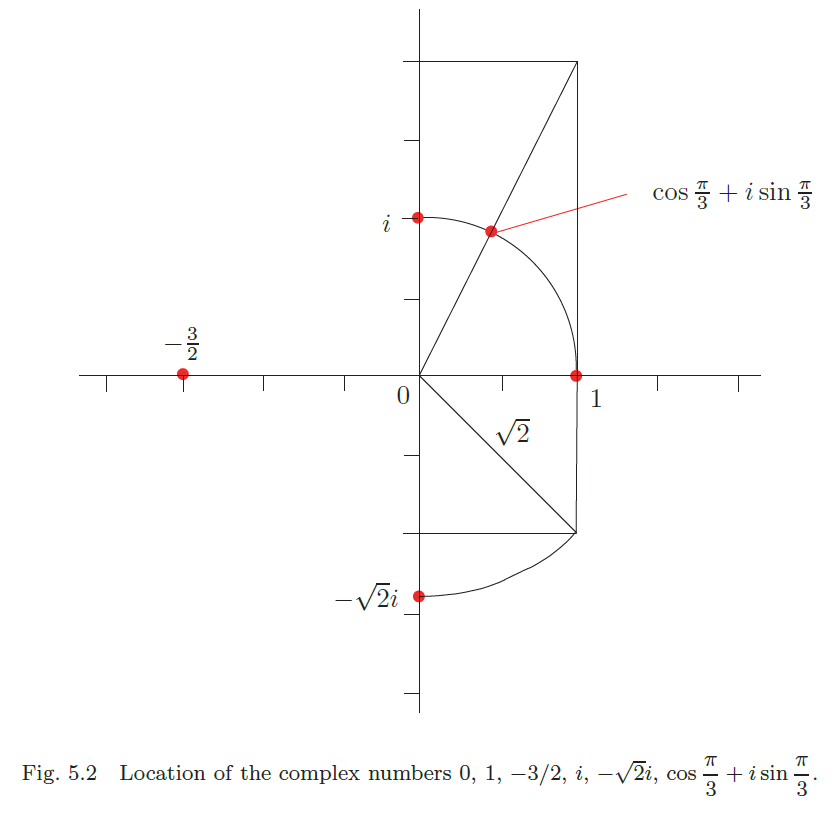
\includegraphics[width=0.65\textwidth]{./Solution/figs/fig-5-2}
\end{center}
\caption{복소수 $0$, $1$, $-3/2$, $i$, $-\sqrt{2}i$,
$\cos\dfrac\pi3 + i\sin\dfrac\pi3$의 위치}
\label{fig-5-2}
\end{figure}

\subsection*{연습문제 \ref{ex-1-5}}

$\theta\in\mathbb R$에 대하여
$(\cos\theta + i\sin\theta)^3 = \cos(3\theta) + i\sin(3\theta)$이다.
\begin{align*}
(\cos\theta + i\sin\theta)^3 
&= (\cos\theta + i\sin\theta)\Big(
(\cos\theta)^2 - (\sin\theta)^2 + i2(\cos\theta)(\sin\theta) \Big) \\
&= (\cos\theta)\left( (\cos\theta)^2 - (\sin\theta)^2 \right)
- (\sin\theta)2(\cos\theta)(\sin\theta)  \\
&\quad\quad + i(\ \cdots\ ).
\end{align*}
따라서 양변의 실수부가 같다는 것을 이용하면,
\begin{align*}
\cos(3\theta) &= \Re((\cos\theta + i\sin\theta)^3) \\
&=(\cos\theta)\left( (\cos\theta)^2 - (\sin\theta)^2 \right)
- 2(\cos\theta)(\sin\theta)^2 \\
&= (\cos\theta)\left( (\cos\theta)^2 - 1 + (\cos\theta)^2 \right)
- 2(\cos\theta)(1-(\cos\theta)^2) \\
&= (\cos\theta)^3 - \cos\theta  + (\cos\theta)^3 - 2\cos\theta + 2(\cos\theta)^3 \\
&= 4(\cos\theta)^3 - 3\cos\theta.
\end{align*}
다른 방법으로, 이항정리 공식
$(a+b)^n = \Sum_{k=0}^n \disp{n \choose k} a^kb^{n-k}$이
복소수 $a,b \in \mathbb C$와 자연수 $n\in \mathbb N$에 대하여
성립한다는 것을 이용하여 보일 수도 있다.
\begin{align*}
\cos(3\theta) &= \Re((\cos\theta + i\sin\theta)^3) \\
&= \Re ( (\cos\theta)^3 + 3(\cos\theta)^2(i\sin\theta) 
+ 3(\cos\theta)(i\sin\theta)^2 + (i\sin\theta)^3) \\
&= (\cos\theta)^3 - 3(\cos\theta)(\sin\theta)^2 \\
&= 4(\cos\theta)^3 - 3\cos\theta.
\end{align*}

\subsection*{연습문제 \ref{ex-1-6}}

$1+i = \sqrt{2}\left(\dfrac1{\sqrt{2}} + i\dfrac1{\sqrt{2}}\right)
= \sqrt{2}\left( \cos\dfrac\pi4 + i\sin \dfrac\pi4 \right)$로 쓸 수 있다.
따라서,
\begin{align*}
(1+i)^{10}
&= (\sqrt{2})^{10} \left( \cos\dfrac\pi4 + i\sin \dfrac\pi4 \right)^{10}
= 2^5 \left( \cos\left(10\cdot \dfrac\pi4\right) 
+ i\sin \left(10\cdot \dfrac\pi4\right) \right) \\
&= 32 \left( \cos\left(2\pi+\dfrac\pi2\right) 
+ i\sin \left(2\pi+\dfrac\pi2\right) \right) \\
&=32 \left( \cos\left(\dfrac\pi2\right) + i\sin \left(\dfrac\pi2\right) \right) 
= 32(0+i\cdot 1) = 32i.
\end{align*}

\subsection*{연습문제 \ref{ex-1-7}}

$2+i$가 실수축의 양의 방향과 이루는 각도는 $\tan^{-1}(1/2)$이고
$3+i$가 실수축의 양의 방향과 이루는 각도는 $\tan^{-1}(1/3)$이다.
따라서, $(2+i)(3+i)$가 실수축의 양의 방향과 이루는 각도는 
$\tan^{-1}(1/2) + \tan^{-1}(1/3)$이다.
한편,
\[
(2+i)(3+i) = 6 - 1 + i(2+3) = 5 + 5i
\]
이므로 $(2+i)(3+i)$가  실수축의 양의 방향과 이루는 각도는
\[
\tan^{-1} (5/5) = \tan^{-1} 1 = \pi/4
\]
이다. 결론적으로, 
$\dfrac\pi4 = \tan^{-1}\dfrac12 + \tan^{-1}\dfrac13$이다.

\subsection*{연습문제 \ref{ex-1-8}}

정삼각형의 꼭지점  $A$, $B$, $C$의 위치가 
반시계방향의 순서로 복소수 $z_A$, $z_B$, $z_C$에 있다고 하자.
$\ell(AC) = \ell(AB)$이고 $\angle CAB=\pi/3$이므로,
\begin{equation}\label{eq-5-9}
z_C - z_A = \left( \cos\dfrac\pi3 + i\sin\dfrac\pi3 \right)(z_B - z_A).
\end{equation}
귀류법을 쓰기 위해 $p,q,m,n\in\mathbb Z$가 
\[
z_C - z_A = p+iq, \quad
z_B - z_A = m+in
\]
을 만족한다고  하자.
그러면, 식 \eqref{eq-5-9}에서
$p+iq = \left(\dfrac12 + \dfrac{\sqrt{3}}2i\right)(m+in)$을 다시 쓰면,
\begin{align}
p &= \dfrac m2 - \dfrac{\sqrt{3}}2n, \label{eq-5-10} \\
q &= \dfrac{m\sqrt{3}}2 + \dfrac n2. \label{eq-5-11}
\end{align}
식 \eqref{eq-5-10}에 $-n$을 곱하고,
식 \eqref{eq-5-11}에 $m$을 곱하여 더하면,
\[
qm - pn = \dfrac{\sqrt{3}}2 (m^2 + n^2)
\]
을 얻는다.
그런데 $m^2+n^2 \ne0$이므로 (즉, $z_B \ne z_A$이므로),
\[
\sqrt{3} = \dfrac{2(qm-pn)}{m^2+n^2} \in \mathbb Q
\]
를 얻어 모순이 생긴다.

\subsection*{연습문제 \ref{ex-1-9}}

$-1 = 1 \cdot (\cos \pi + i \sin \pi)$로 쓸 수 있다.
$w = \rho(\cos\alpha + i\sin\alpha)$가 
\[
w^4 = \rho^4(\cos(4\alpha) + i\sin(4\alpha)) = 1 \cdot (\cos \pi + i \sin \pi)
\]
를 만족해야 하므로,
$\rho^4 = 1$에서 $\rho=1$이다.
또한, $4\alpha \in \{ \pi, \pi\pm2\pi, \pi\pm4\pi, \ldots\}$에서
\[
\alpha \in \left\{ \dfrac\pi4, \dfrac\pi4\pm\dfrac\pi2, \dfrac\pi4\pm\pi,\ldots
\right\}.
\]
따라서 $ w = \rho(\cos\alpha + i\sin\alpha) = 1\cdot((\cos\alpha + i\sin\alpha) $는
다음 집합에 속한다.
\begin{align*}
&\left\{ \cos\dfrac\pi4+i\sin\dfrac\pi4,\ \cos\dfrac{3\pi}4+i\sin\dfrac{3\pi}4, \
\cos\dfrac{5\pi}4+i\sin\dfrac{5\pi}4, \ \cos\dfrac{7\pi}4+i\sin\dfrac{7\pi}4
\right\} \\
&\qquad\quad\quad = \left\{ \dfrac{1+i}{\sqrt{2}},  \ \dfrac{-1+i}{\sqrt{2}}, \
 \dfrac{-1-i}{\sqrt{2}}, \ \dfrac{1-i}{\sqrt{2}} \right\}.
\end{align*}

네 개의 해를 복소평면에 그려보면 그림 \ref{fig-5-3}\과 같다.

\begin{figure}[h!]
\begin{center}
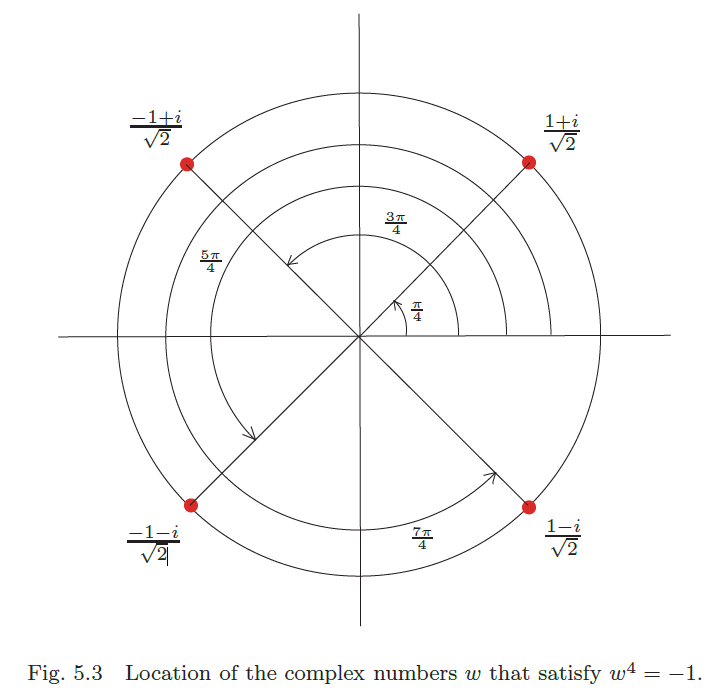
\includegraphics[width=0.65\textwidth]{./Solution/figs/fig-5-3}
\end{center}
\caption{$w^4=-1$을 만족하는 복소수 $w$의 위치}
\label{fig-5-3}
\end{figure}

\subsection*{연습문제 \ref{ex-1-10}}

방정식으로부터
\[
0=z^6 -z^3-2 = (z^3)^2 -2z^3 +z^3 -2 = (z^3-2)(z^3+1)
\]
이므로
$z^3=2$ 또는 $z^3=-1$이다.
$z^3=2$를 만족하는 해를 구하면
\[
z\in \left\{ \sqrt[3]{2} \left( \cos\dfrac{2\pi}3 + i\sin\dfrac{2\pi}3\right), \
\sqrt[3]{2} \left( \cos\dfrac{4\pi}3 + i\sin\dfrac{4\pi}3\right),  \
\sqrt[3]{2} \right\}
\]
로부터 
\[
z\in \left\{ \sqrt[3]{2} \left( - \dfrac12+ i\dfrac{\sqrt{3}}2\right), \
\sqrt[3]{2} \left( -\dfrac12 - i\dfrac{\sqrt{3}}2\right),  \
\sqrt[3]{2} \right\}
\]
이다. 한편, $z^3=-1$의 해는
\[
z\in\left\{ \cos\dfrac\pi3 + i\sin\dfrac\pi3,\  \cos\pi + i\sin\pi, \
\cos\dfrac{5\pi}3 + i\sin\dfrac{5\pi}3 \right\}
\]
로부터 
\[
z\in \left\{ \dfrac12+ i\dfrac{\sqrt{3}}2, \ -1, \
\dfrac12 - i\dfrac{\sqrt{3}}2 \right\}
\]
이다. 결론적으로
$z^6 - z^3-2=0$일 필요충분조건은 [$z^3=2$ 또는 $z^3=-1$]이다.
즉,
\begin{align*}
z\in & \left\{ \sqrt[3]{2} \left( - \dfrac12+ i\dfrac{\sqrt{3}}2\right), \
\sqrt[3]{2} \left( -\dfrac12 - i\dfrac{\sqrt{3}}2\right), \
\sqrt[3]{2} \right\}\\
&\bigcup \left\{ \dfrac12+ i\dfrac{\sqrt{3}}2,\ -1, \
\dfrac12 - i\dfrac{\sqrt{3}}2 \right\}.
\end{align*}
따라서 구하는 해는
\[
z\in \left\{ \sqrt[3]{2} \left( - \dfrac12+ i\dfrac{\sqrt{3}}2\right), \
\sqrt[3]{2} \left( -\dfrac12 - i\dfrac{\sqrt{3}}2\right), \
\sqrt[3]{2}, \
\dfrac12+ i\dfrac{\sqrt{3}}2, \ -1, \
\dfrac12 - i\dfrac{\sqrt{3}}2 \right\}.
\]

\subsection*{연습문제 \ref{ex-1-11}}

$\omega^3=1$을 만족하는 $\omega\in\mathbb C \setminus \mathbb R$을 생각하자.
그러면, $(\omega-1)(\omega^2+\omega+1)=0$이고,
$\omega\ne1$이므로 $\omega^2+\omega+1=0$이다.
따라서,
\begin{align*}
((b-a)\omega &+(b-c))((b-a)\omega^2+(b-c)) \\
&= (b-a)^2\omega^3 + (b-a)(b-c)(-1) + (b-c)^2 \\
&= (b-a)^2\cdot 1 + (b-a)(b-c)(-1)  + (b-c)^2 \\
&= (b-a)(b-a-b+c) + (b-c)^2 \\
&=bc-ca-ab+a^2+b^2-2bc+c^2 \\
&= a^2+b^2+c^2 -ab - bc - ca = 0.
\end{align*}
따라서 $(b-a)\omega = c-b$이거나 $(b-a)\omega^2 = c-b$이다.
두번째 식은 $(b-a)\omega^3 = (c-b)\omega$와 동치이므로
$(c-b)\omega = b-a$이다.
이로부터 $|b-a|=|c-b|$를 얻고
$a$와 $b$, $a$와 $c$를 잇는 두 선분의 사잇각은 $\pi/3$이다.
그림 \ref{fig-5-4}\를 참고하라.

\begin{figure}[h!]
\begin{center}
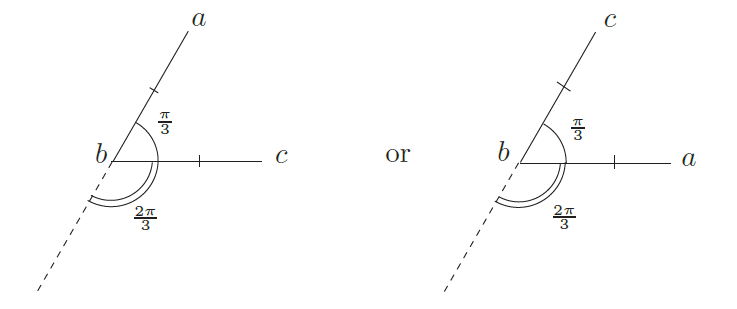
\includegraphics[width=0.6\textwidth]{./Solution/figs/fig-5-4}
\end{center}
\caption{정삼각형을 이루는 세 점 $a$, $b$, $c$}
\label{fig-5-4}
\end{figure}

두 가지 그림 모두 세 점 $a$, $b$, $c$는 정삼각형을 이룬다.
 $a$, $b$, $c$가 실수인 경우는 한점 $r\in\mathbb R$로 모이게 되어
 $a=b=c(=r)$이 되어 실수의 경우도 원하는 결과를 얻는다.

\subsection*{연습문제 \ref{ex-1-12}}

$\omega\in\mathbb C\setminus \mathbb R$이 $\omega^3=1$을 만족한다고 하자.
$(\omega-1)(\omega^2+\omega+1)=0$이고,
$\omega\ne1$이므로 $\omega^2+\omega+1=0$이다.
또한, $1+\omega^2+\omega^4 = 1+ \omega^2 + \omega\cdot\omega^3 =
1+ \omega^2 + \omega = 0$이므로,
\[
(1+1)^{3n} + (1+\omega)^{3n} + (1+\omega^2)^{3n}
= \Sum_{k=0}^{3n} {3n \choose k} (1+\omega^k + \omega^{2k}).
\]
그런데,
\begin{align*}
(1+\omega^k + \omega^{2k})
&= \begin{cases}
1+1+1, & k\equiv 0 \mod 3, \\
1+\omega + \omega^2, & k\equiv 1 \mod 3, \\
1+\omega^2 + \omega^4,& k\equiv 2 \mod 3
\end{cases} \\
&=\begin{cases}
3, & k\equiv 0 \mod 3, \\
0, & k\equiv 1 \mod 3, \\
0, & k\equiv 2 \mod 3.
\end{cases}
\end{align*}
따라서
\[
(1+1)^{3n} + (1+\omega)^{3n} + (1+\omega^2)^{3n}
= 3\cdot \left(
{3n \choose 0} + {3n \choose 3} + \cdots + {3n \choose 3n} \right).
\]
다른 방법으로 보면,
\begin{align*}
(1+1)^{3n} + (1+\omega)^{3n} + (1+\omega^2)^{3n}
&= 2^{3n} + (-\omega^2)^{3n} +  (-\omega)^{3n} \\
&= 2^{3n} + (-1)^n + (-1)^n \\
&= 2^{3n} + 2\cdot(-1)^n
\end{align*}
이므로 원하는 결과를 얻는다.

\subsection*{연습문제 \ref{ex-1-13}}



그림 \ref{fig-5-5}\와 같이
평면위의 네 점 $A$, $B$, $C$, $D$를 복소수 $a$, $b$, $c$, $d$에 각각 대응시키자.
$AB'$은  $A$를 중심으로 하여 $AB$를 반시계방향으로 $90^\circ$회전한 것이므로
$B'$은 복소수 $a-i(b-a)$에 대응된다.
$P$는 $BB'$의 중점이므로 다음 복소수에 대응된다.
\[
\dfrac{a+b-i(b-a)}2.
\]
같은 방법으로 $Q$, $R$, $S$는 각각 다음 복소수에 대응된다.
\[
\dfrac{b+c-i(c-b)}2, \quad
\dfrac{c+d-i(d-c)}2, \quad
\dfrac{d+a-i(a-d)}2.
\]
점 $P$, $Q$, $R$, $S$에 대응되는 복소수를 각각
$p$, $q$, $r$, $s$라 하면,
\begin{align*}
i(q-s) &= i \left(
\dfrac{b+c-i(c-b)}2 - \dfrac{d+a-i(a-d)}2 \right) \\
&= \dfrac{-b+c-a+d+i(b+c-d-a)}2 \\
&= \dfrac{-a-b+i(b-a)}2 + \dfrac{c+d-i(d-c)}2 = -p+r
\end{align*}
이므로, $|q-s| = |p-r|$이 되어 $\ell(QS) = \ell(PR)$이다.
또한, $i$를 곱하는 것은 원점을 중심으로 $90^\circ$ 회전을 의미하기 때문에
$PR\perp QS$이다.

\begin{figure}[h!]
\begin{center}
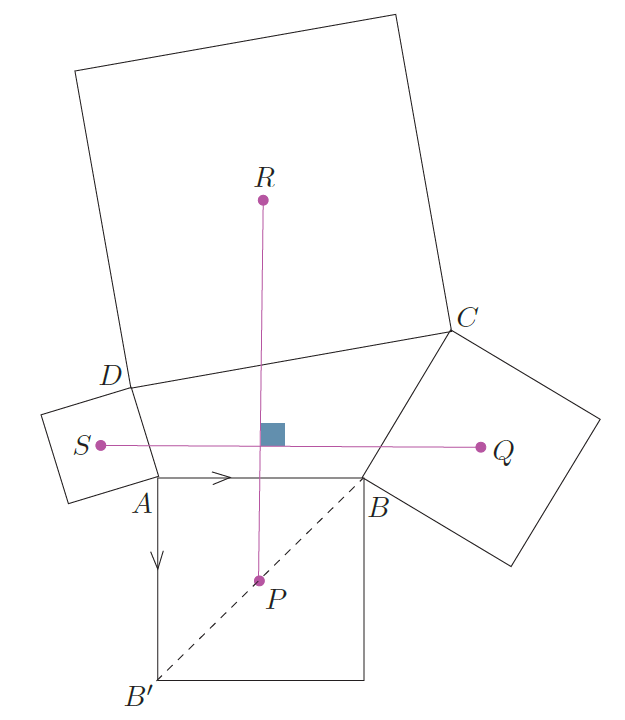
\includegraphics[width=0.5\textwidth]{./Solution/figs/fig-5-5}
\end{center}
\caption{$RP$와 $SQ$는 길이가 같고 수직으로 만난다}
\label{fig-5-5}
\end{figure}

\subsection*{연습문제 \ref{ex-1-14}}

실수 $x_1, x_2, y_1, y_2$에 대하여
$z_1 = x_1 + iy_1$, $z_2 = x_2 + iy_2$라 하자.
그러면 $z_1z_2 = x_1x_2 - y_1y_2 + i(x_1y_2+y_1x_2)$이고,
\begin{align*}
|z_1z_2|^2 &=  (x_1x_2 - y_1y_2)^2 + (x_1y_2 + y_1x_2)^2 \\
&= x_1^2x_2^2 - \cancel{2x_1x_2y_1y_2} + y_1^2y_2^2
+ x_1^2y_2^2 + \cancel{2x_1y_2y_1x_2} + y_1^2x_2^2 \\
&=x_1^2(x_2^2+y_2^2) + y_1^2(y_2^2+x_2^2)
= (x_1^2+y_1^2)(x_2^2+y_2^2) \\
&= |z_1|^2|z_2|^2.
\end{align*}
$|z_1|$, $|z_2|$, $|z_1z_2|$는 모두 음이 아닌 실수이므로
$|z_1||z_2| = |z_1||z_2|$가 성립한다.

\subsection*{연습문제 \ref{ex-1-15}}

$z=x+iy$ ($x,y\in\mathbb R$)이라 하자. 그러면,
\[
\overline{(\bar z)} = \overline{x-iy}
= x - i(-y) = x+iy = z.
\]
또한, $z\bar z = (x+iy)(x-iy) = x^2+y^2 + i(- xy + xy)
= x^2+y^2 = |z|^2$.

끝으로,
\begin{align*}
\dfrac{z + \bar z}2 &= \dfrac{x+\cancel{iy}+ x -\cancel{iy}}2
= \dfrac{2x}2 = x =\Re(z), \\
\dfrac{z - \bar z}{2i} &= \dfrac{\cancel{x}+iy - \cancel{x} +iy}{2i}
= \dfrac{2iy}{2i} = y = \Im(z).
\end{align*}

\subsection*{연습문제 \ref{ex-1-16}}

$z = x+iy$ ($x,y\in\mathbb R$)이라 하면,
\begin{align*}
|z| &= |x+iy| = \sqrt{x^2+y^2} = \sqrt{x^2+(-y)^2} = |x-iy| = |\bar z|, \\
|\Re(z)| & =  |x| = \sqrt{x^2} \le  \sqrt{x^2+y^2} = |x+iy| = |z|, \\
|\Im(z)| &= |y| = \sqrt{y^2} \le  \sqrt{x^2+y^2} = |x+iy| = |z|.
\end{align*}

$\bar z$는 $z$를 실수축에 대칭시켜 얻어지며,
$0\in\mathbb R$이므로 원점과 $z$와의 거리는 $\bar z$와의 거리와 같다.
즉, $ |z| = |\bar z|$.
부등식 $|\Re(z)| \le|z|$와 $|\Im(z)|\le |z|$는 
아래 그림에서 직각삼각형에서 빗변의 길이가 가장 길다는 것을 의미한다.

\begin{figure*}[h!]
\begin{center}
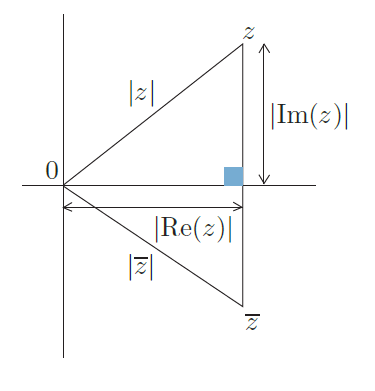
\includegraphics[width=0.4\textwidth]{./Solution/figs/fig-s-0-1}
\end{center}
%\caption{$RP$와 $SQ$는 길이가 같고 수직으로 만난다}
%\label{fig-5-5}
\end{figure*}

\subsection*{연습문제 \ref{ex-1-17}}

우선 $|\bar az| = |\bar a||z| = |a||z| <1\cdot 1 =1$이므로, $\bar az \ne 1$이고,
\begin{align*}
\dfrac{z-a}{1-\bar az}\cdot \overline{\left(\dfrac{z-a}{1-\bar az}\right)}
&= \dfrac{z-a}{1-\bar az}\cdot \dfrac{\bar z-\bar a}{1-a\bar z}
= \dfrac{z\bar z - a\bar z - \bar a z+a\bar a}{1-a\bar z - \bar a z + a\bar a z \bar z} \\
&= \dfrac{|z|^2 - a\bar z - \bar a z + |a|^2}{1-a\bar z - \bar a z + |a|^2|z|^2} \\
&= \dfrac{1 - a\bar z - \bar a z + |a|^2|z|^2+|z|^2+|a|^2-1-|a|^2|z|^2}
{1-a\bar z - \bar a z + |a|^2|z|^2} \\
&= 1 + \dfrac{|z|^2+|a|^2-1-|a|^2|z|^2}{1-a\bar z - \bar a z + |a|^2|z|^2} \\
&= 1 + \dfrac{|z|^2+|a|^2-1-|a|^2|z|^2}{|1- \bar a z|^2} \\
&= 1 -  \dfrac{(1-|z|^2)(1-|a|^2)}{|1- \bar a z|^2}.
\end{align*}
따라서
$\left| \dfrac{z-a}{1-\bar az} \right|^2 = 1 -
\underbrace{\dfrac{(1-|z|^2)(1-|a|^2)}{|1- \bar a z|^2}}_{\ge0\ (|z|\le 1, |a|<1\text{ 이므로})}
\le 1-0 = 1$.

\subsection*{연습문제 \ref{ex-1-18}}

$w\in\mathbb C$가 $p(w)=0$, 즉,
$c_0 + c_1w + \cdots + c_dw^d=0$을 만족한다고 하자. 
그러면,
\[
\overline{c_0 + c_1w + \cdots + c_dw^d} = \bar 0 = 0
\]
이고, 모든 $c_k$ ($0\le k\le d$)가 실수이므로
\begin{align*}
0 & = \overline{c_0 + c_1w + \cdots + c_dw^d} 
= \overline{c_0} + \overline{c_1w} + \cdots + \overline{c_dw^d} \\
&= \overline{c_0} + \overline{c_1}\overline{w} + \cdots + \overline{c_d}\overline{w^d}
= c_0 + c_1\overline{w} + \cdots + c_d(\bar w)^d.
\end{align*}
마지막 등식에서 
\[
\overline{w^k} = \underbrace{\overline{w\cdots w}}_{k\text{번}}
= \underbrace{\bar w \cdots \bar w}_{k\text{번}}
= (\bar w)^k,
\quad 1\le k \le d
\]
를 사용하였다.
따라서, $0=c_0 + c_1\overline{w} + \cdots + c_d(\bar w)^d = p(\bar w)$.

\subsection*{연습문제 \ref{ex-1-19}}

$a = |a|(\cos\alpha + i\sin\alpha)$, 
$b = |b|(\cos\beta + i\sin \beta)$라고 하자.
단, $\alpha, \beta \in [0,2\pi)$. 그러면,
\begin{align*}
a\bar b &= |a|(\cos\alpha + i\sin\alpha)\cdot
|b|(\cos\beta - i\sin \beta) \\
&=|a||b|(\cos\alpha + i\sin\alpha)(\cos\beta - i\sin \beta)
\end{align*}
이고 $\Im(a\bar b) = |a||b|(-(\cos\alpha)(\sin\beta) + (\sin\alpha)(\cos\beta))
= |a||b|\sin(\alpha-\beta)$.

$0$, $a$, $b$를 꼭지점으로 하는 $\Delta OAB$의 면적은
($O\equiv 0$, $A\equiv a$, $B\equiv b$)
\[
\dfrac12 \ell(OA)\ell(OB) \cdot \sin \angle AOB
= \dfrac12 |a|\cdot |b| \cdot |\sin(\alpha-\beta)|
= \dfrac12 |\Im(a\bar b)| = \left| \dfrac{\Im(a\bar b)}2\right|.
\]

\begin{figure}[h!]
\begin{center}
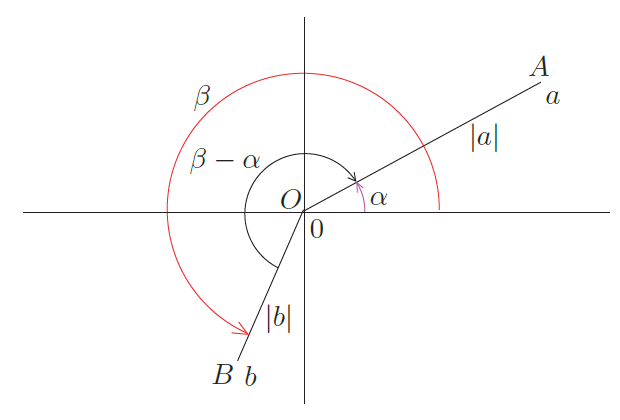
\includegraphics[width=0.5\textwidth]{./Solution/figs/fig-5-6}
\end{center}
\caption{$0$, $a$, $b$를 꼭지점으로 하는 $\Delta OAB$의 면적}
\label{fig-5-6}
\end{figure}

\subsection*{연습문제 \ref{ex-1-20}}

$z_1, z_2, z_3 \in\mathbb C$에 대하여,
\[
w:= \overline{i\cdot \det \begin{bmatrix}
1 & z_1 & \overline{z_1} \\
1 & z_2 & \overline{z_2} \\
1 & z_3 & \overline{z_3}
\end{bmatrix}}
= -i\cdot \overline{\det \begin{bmatrix}
1 & z_1 & \overline{z_1} \\
1 & z_2 & \overline{z_2} \\
1 & z_3 & \overline{z_3}
\end{bmatrix}}.
\]
한편, 정사각행렬 $M=[m_{ij}]$에 대하여,
\[
\det M = \sum_{\sigma\in S_n} (\sgn \sigma) \cdot m_{i\sigma(i)},
\]
여기서, $S_n$은 $\{1,\ldots, n\}$에 대한 모든 치환(permutation)의 집합이다.
\[
\overline{\det M} = \sum_{\sigma\in S_n} (\sgn \sigma) \cdot
\overline{m_{i\sigma(i)}} = \det \overline{M},
\]
여기서, $\overline{M}$은 $M$의 모든 원소에 대하여 켤레복소수를 취한 것이다.
따라서,
\[
\overline{\det \begin{bmatrix}
1 & z_1 & \overline{z_1} \\
1 & z_2 & \overline{z_2} \\
1 & z_3 & \overline{z_3}
\end{bmatrix}}
= \det \begin{bmatrix}
1 & \overline{z_1} & z_1 \\
1 & \overline{z_2} & z_2 \\
1 & \overline{z_3} & z_3
\end{bmatrix}
= -  \det \begin{bmatrix}
1 & z_1 & \overline{z_1} \\
1 & z_2 & \overline{z_2} \\
1 & z_3 & \overline{z_3}
\end{bmatrix},
\]
마지막 등식은 두번째 열과 세번째 열을 바꾼 것이다.
종합하면,
\begin{align*}
\overline{i\cdot \det \begin{bmatrix}
1 & z_1 & \overline{z_1} \\
1 & z_2 & \overline{z_2} \\
1 & z_3 & \overline{z_3}
\end{bmatrix}}
= -i\cdot \overline{\det \begin{bmatrix}
1 & z_1 & \overline{z_1} \\
1 & z_2 & \overline{z_2} \\
1 & z_3 & \overline{z_3}
\end{bmatrix}}
& = -i \cdot \left(
-  \det \begin{bmatrix}
1 & z_1 & \overline{z_1} \\
1 & z_2 & \overline{z_2} \\
1 & z_3 & \overline{z_3}
\end{bmatrix}
\right) \\
& = i \cdot  \det \begin{bmatrix}
1 & z_1 & \overline{z_1} \\
1 & z_2 & \overline{z_2} \\
1 & z_3 & \overline{z_3}
\end{bmatrix}.
\end{align*}
따라서, $w$는 켤레복소수와 동일하므로 실수이다.

\subsection*{연습문제 \ref{ex-1-21}}

\begin{align*}
|z_1+z_2|^2 + & |z_1 - z_2|^2 \\
&= (z_1 + z_2)(\overline{z_1} + \overline{z_2}) + (z_1 - z_2)(\overline{z_1} - \overline{z_2}) \\
&= z_1\cdot \overline{z_1} + z_1 \cdot \overline{z_2} + z_2 \cdot \overline{z_1}
+ z_2\cdot \overline{z_2} \\
&\qquad + z_1\overline{z_1} + z_1\cdot(-\overline{z_2}) + (-z_2)\cdot\overline{z_1}
+ (-z_2)(-\overline{z_2}) \\
& = |z_1|^2 + \cancel{z_1 \cdot \overline{z_2}} + \cancel{z_2 \cdot \overline{z_1}}
+ |z_2|^2 + |z_1|^2 - \cancel{z_1 \cdot \overline{z_2}}  
- \cancel{z_2 \cdot \overline{z_1}} + |z_2|^2 \\
&= 2(|z_1|^2 + |z_2|^2).
\end{align*}

복소평면에서 $0$, $z_1$, $z_2$, $z_1+z_2$를 꼭지점으로 하는 평행사변형 $P$를 생각하자.
그러면, $|z_1+z_2|$는 $P$의 한쪽 대각선의 길이가 되고,
$|z_1-z_2|$는 다른쪽 대각선의 길이가 된다. 또한, $|z_1|$, $|z_2|$는
$P$의 두변의 길이다. 따라서 위의 식이 의미하는 것은
``평행사변형에서 대각선 길이의 제곱의 합은 변의 길이의 제곱의 합의 두배와 같다'' 이다.

\subsection*{연습문제 \ref{ex-1-22}}

$z_1, z_2\in\mathbb C$에 대하여,
$|z_1| = |z_1 - z_2 + z_2| \le |z_1 - z_2| + |z_2|$이므로
\begin{equation} \label{eq-5-12}
|z_1| - |z_2| \le |z_1 - z_2|.
\end{equation}
모든 $z_1, z_2\in\mathbb C$에 대하여,
식 \eqref{eq-5-12}에서 $z_1$과 $z_2$의 역할을 바꾸어도 성립하므로
\begin{equation}\label{eq-5-13}
|z_2| - |z_1| \le |z_2 - z_1| = |-(z_1-z_2)|
= |-1| |z_1-z_2| =|z_1-z_2|.
\end{equation}
식 \ref{eq-5-12}\와 \ref{eq-5-13}\로부터 
$\big| |z_1| -|z_2| \big| \le |z_1 - z_2|$이다.

\subsection*{연습문제 \ref{ex-1-23}}

\begin{itemize}
\item[(1),(2),(3):] \
\begin{figure}[h!]
\begin{center}
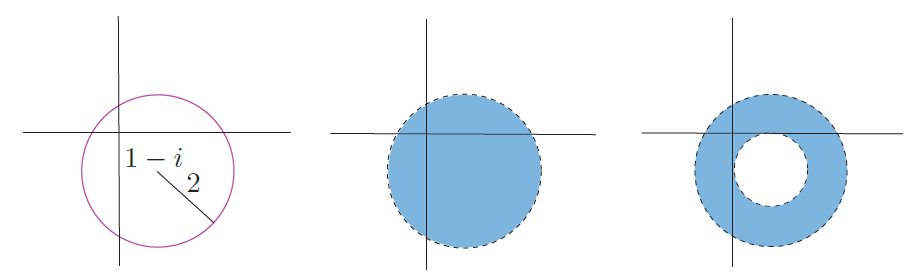
\includegraphics[width=0.8\textwidth]{./Solution/figs/fig-5-7}
\end{center}
\caption{왼쪽부터 $|z-(1-i)|=2$, $|z-(1-i)|<2$,
$1<|z-(1-i)|<2$}
\label{fig-5-7}
\end{figure}
\item[(4):] $z=x+iy$ ($x,y\in\mathbb R$)이라 하면,
$\Re(z-(1-i))=3$은 $x-1=3$과 동치이므로, $x=4$이다.
\begin{figure*}[h!]
\begin{center}
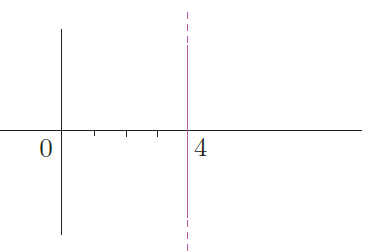
\includegraphics[width=0.3\textwidth]{./Solution/figs/fig-s-0-2}
\end{center}
%\caption{$RP$와 $SQ$는 길이가 같고 수직으로 만난다}
%\label{fig-5-5}
\end{figure*}
\item[(5):] $z=x+iy$ ($x,y\in\mathbb R$)이라 하면,
$|\Im(z-(1-i))|<3$은 $|y+1|<3$, 즉, $-4<y<2$와 같다.
\begin{figure*}[h!]
\begin{center}
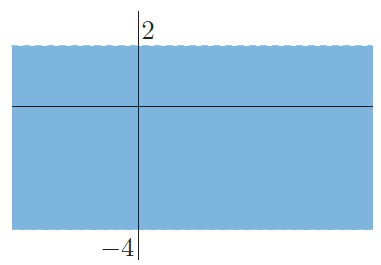
\includegraphics[width=0.3\textwidth]{./Solution/figs/fig-s-0-3}
\end{center}
%\caption{$RP$와 $SQ$는 길이가 같고 수직으로 만난다}
%\label{fig-5-5}
\end{figure*}
\item[(6):] $\{ z\in\mathbb C\,:\, |z-(1-i)| = |z-(1+i)|\}$는
$1-i$와 $1+i$에서 같은 거리에 있는 복소수 $z$의 집합이다.
따라서, $1-i$와 $1+i$을 잇는 선분의 수직이등분선이 된다.
즉, 실수축이다.
\begin{figure}[h!]
\begin{center}
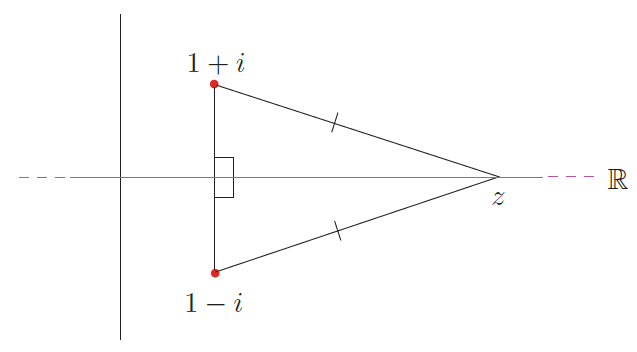
\includegraphics[width=0.5\textwidth]{./Solution/figs/fig-5-8}
\end{center}
\caption{$|z-(1-i)| = |z-(1+i)|$를 만족하는 집합은 $\mathbb R$}
\label{fig-5-8}
\end{figure}
\item[(7):] 방정식 $|z-(1-i)| + |z-(1+i)| =2$는 
$z$에서 $1+i$까지의  거리와  $1-i$까지의 거리의 합이 $2$가 됨을 의미한다.
그런데 $1-i$와 $1+i$의 거리가 $2$이므로
$z$는 $1-i$와 $1+i$를 잇는 선분에 있다.

\begin{figure}[h!]
\begin{center}
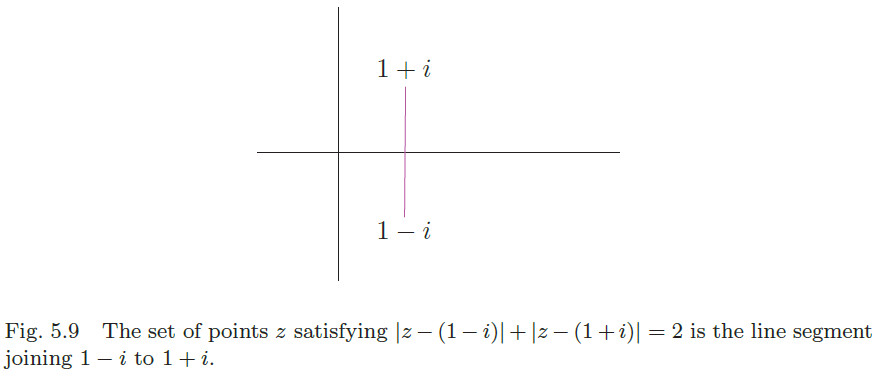
\includegraphics[width=0.3\textwidth]{./Solution/figs/fig-5-9}
\end{center}
\caption{$|z-(1-i)| + |z-(1+i)|=2$를 만족하는 집합은 $1-i$와 $1+i$를 잇는 선분이다.}
\label{fig-5-9}
\end{figure}

직접 계산하는 방식으로도 같은 결과를 얻을 수 있다.
$z=x+iy$ ($x,y\in\mathbb R$)이면
\begin{align*}
2 &= \sqrt{(x-1)^2 + (y+1)^2} + \sqrt{(x-1)^2 + (y-1)^2} \\
&\ge |y+1| + |y-1| \ge 1 + \cancel{y} + 1 - \cancel{y} =2
\end{align*}
이므로 $|y+1| + |y-1|=2$이고, $x=1$이다.

\item[(8):] 방정식 $|z-(1-i)| + |z-(1+i)| =3$을 만족하는 집합은
초점이 $1+i$와 $1-i$인 타원 $E$이 된다.
따라서, $\{z\in\mathbb C\,:\, |z-(1-i)| + |z-(1+i)| < 3\}$은
타원 $E$의 내부가 된다.
\begin{figure}[h!]
\begin{center}
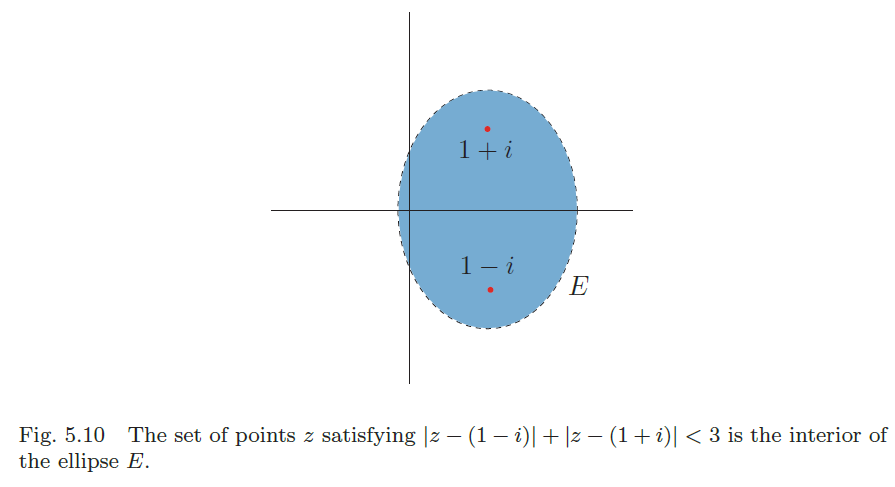
\includegraphics[width=0.3\textwidth]{./Solution/figs/fig-5-10}
\end{center}
\caption{$|z-(1-i)| + |z-(1+i)| < 3$을 만족하는 집합은 타원  $E$의 내부이다.}
\label{fig-5-10}
\end{figure}
\end{itemize}

\subsection*{연습문제 \ref{ex-1-24}}

$z\ne0$에 대하여
$p(z) = z^d \left( c_d + \dfrac{c_{d-1}}z + \cdots + \dfrac{c_1}{z^{d-1}}
+ \dfrac{c_0}{z^d} \right)$.
\[
\lim_{n\to\infty}  \left( 
 \dfrac{|c_{d-1}|}n + \cdots + \dfrac{|c_1|}{n^{d-1}}
+ \dfrac{|c_0|}{n^d} \right) = 0
\]
이므로, 
다음을  만족하도록 충분히 큰 $N$을 잡을 수 있다.
\[
\dfrac{|c_{d-1}|}N + \cdots + \dfrac{|c_1|}{N^{d-1}}
+ \dfrac{|c_0|}{N^d} < \dfrac{|c_d|}2.
\]
그러면 $|z|>N=:R$에 대하여
\begin{align*}
|p(z)| &= |z^d| \left|
c_d + \dfrac{c_{d-1}}z + \cdots + \dfrac{c_1}{z^{d-1}}
+ \dfrac{c_0}{z^d} \right| \\
&\ge |z|^d \left( |c_d| - \left| \dfrac{c_{d-1}}z + \cdots + \dfrac{c_1}{z^{d-1}}
+ \dfrac{c_0}{z^d} \right| \right) \\
&\ge |z|^d \left(|c_d| - \left( \dfrac{|c_{d-1}|}{|z|} + \cdots + \dfrac{|c_1|}{|z|^{d-1}}
+ \dfrac{|c_0|}{|z|^d} \right) \right) \\
&\ge |z|^d \left(|c_d| - \left( \dfrac{|c_{d-1}|}N + \cdots + \dfrac{|c_1|}{N^{d-1}}
+ \dfrac{|c_0|}{N^d} \right) \right) \\
&\ge |z|^d \left(|c_d| - \dfrac{|c_d|}2 \right) = \underbrace{\dfrac{|c_d|}2}_{=:M} |z|^d.
\end{align*}

\subsection*{연습문제 \ref{ex-1-25}}

$(\Leftarrow):$ \\[1ex]
실수열 $(\Re(z_n))_{n\in\mathbb N}$과 
$(\Im(z_n))_{n\in\mathbb N}$이 각각 $\Re(L)$과 $\Im(L)$로 수렴한다고 하자.
그러면, 주어진 $\epsilon>0$에 대하여,
충분히 큰 $N$이 존재하여 $n>N$이면
\[
|\Re(z_n) - \Re(L)| < \dfrac\epsilon{\sqrt{2}},\quad
|\Im(z_n) - \Im(L)| < \dfrac\epsilon{\sqrt{2}}
\]
을 만족하게 할 수 있고,
\begin{align*}
|z_n-L| &= \sqrt{ (\Re(z_n) - \Re(L))^2 + (\Im(z_n) - \Im(L))^2} \\
&< \sqrt{\left(\dfrac\epsilon{\sqrt{2}}\right)^2  + \left(\dfrac\epsilon{\sqrt{2}}\right)^2}
= \epsilon.
\end{align*}
따라서 $(z_n)_{n\in\mathbb N}$은 $L$로 수렴한다.

\noindent $(\Rightarrow):$\\[1ex]
$(z_n)_{n\in\mathbb N}$이 $L$로 수렴한다고 가정하자.
$n>N$이면  $|z-L|<\epsilon$이 되도록 하는 $N$을 잡을 수 있다.
그러면 모든 $n>N$에 대하여,
\begin{align*}
|\Re(z_n) - \Re(L)| &= |\Re(z_n -L)| \le |z_n -L| <\epsilon, \\
|\Im(z_n) - \Re(L)| &= |\Im(z_n -L)| \le |z_n -L| <\epsilon
\end{align*}
이 되어
$(\Re(z_n))_{n\in\mathbb N}$과 
$(\Im(z_n))_{n\in\mathbb N}$이 각각 
$\Re(L)$과 $\Im(L)$로 수렴한다.

\subsection*{연습문제 \ref{ex-1-26}}

$(\Rightarrow):$\\[1ex]
$(z_n)_{n\in\mathbb N}$이 $L$로 수렴한다고 가정하자.
그러면 $(\Re(z_n))_{n\in\mathbb N}$과 
$(\Im(z_n))_{n\in\mathbb N}$이 각각 
$\Re(L)$과 $\Im(L)$로 수렴한다.
따라서 $(\Re(z_n))_{n\in\mathbb N}$과 
$(-\Im(z_n))_{n\in\mathbb N}$은 각각 
$\Re(L)$과 $-\Im(L)$로 수렴한다.
즉, $(\Re(\overline{z_n}))_{n\in\mathbb N}$와
$(\Im(\overline{z_n}))_{n\in\mathbb N}$가 각각 
$\Re(\overline{L})$와 $\Im(\overline{L})$로 수렴한다.
결론적으로 $(\overline{z_n})_{n\in\mathbb N}$가 $\overline{L}$로 수렴한다.

\noindent $(\Leftarrow):$ \\[1ex]
$(\overline{z_n})_{n\in\mathbb N}$이 $\overline{L}$로 수렴한다고 하자.
앞의 증명에서 $(\overline{(\overline{z_n})})_{n\in\mathbb N}$이 
$\overline{(\overline{L})}$로 수렴한다.
다시 쓰면, $(z_n)_{n\in\mathbb N}$이 $L$로 수렴한다.

\subsection*{연습문제 \ref{ex-1-27}}

$(z_n)_{n\in\mathbb N}$이 $\mathbb C$의 코시수열이라고 하자.
\begin{align*}
|\Re(z_n) - \Re(z_m)| &= |\Re(z_n-z_m)| \le |z_n - z_m|, \\
|\Im(z_n) - \Im(z_m)| &= |\Im(z_n-z_m)| \le |z_n - z_m|
\end{align*}
이므로  $(\Re(z_n))_{n\in\mathbb N}$과 
$(\Im(z_n))_{n\in\mathbb N}$도 코시수열이다.
$\mathbb R$의 완비성으로부터 두 수열은 수렴한다.
각각 $a,b\in\mathbb R$로 수렴한다고 하자.
그러면 $(z_n)_{n\in\mathbb N}$은 $\mathbb C$에서 $a+ib$로 수렴한다.
따라서 $\mathbb C$는 완비공간이다.

\subsection*{연습문제 \ref{ex-1-28}}

$z_0\in\mathbb C$와 $\epsilon >0$이 주어졌다고 하자.
$\delta = \epsilon>0$으로 잡으면,
$|z-z_0|< \delta$일 때,
\[
|\Re(z) - \Re(z_0)| = |\Re(z-z_0)| \le |z-z_0| < \delta = \epsilon
\]
을 만족한다.
따라서 $z \mapsto \Re(z)$는 $z_0$에서 연속이고,
$z_0\in\mathbb C$는 임의로 선택할 수 있으므로
$z \mapsto \Re(z)$는 $\mathbb C$에서 연속이다.

\subsection*{연습문제 \ref{ex-1-29}}

$U:= \{ z\in\mathbb C\,:\, \Re(z)\cdot \Im(z) >1 \}$이라 하자.
$U$의 여집합을 $F:=U^C$로 쓰자.
$F$에 정의된 수열 $(z_n)_{n\in\mathbb N}$이 $\mathbb C$에서 $L$로 수렴한다면,
\begin{equation} \label{eq-5-14}
\Re(z_n)\cdot \Im(z_n) \le 1
\quad (n\in \mathbb N)
\end{equation}
이고 $(\Re(z_n))_{n\in\mathbb N}$과 
$(\Im(z_n))_{n\in\mathbb N}$이 각각 $\Re(L)$과 $\Im(L)$로 수렴한다.
따라서,  $(\Re(z_n)\cdot \Im(z_n))_{n\in\mathbb N}$도 수렴하며
극한은 $\Re(L)\cdot \Im(L)$이 된다.
식 \eqref{eq-5-14}\로부터 $\Re(z)\cdot \Im(z) \le 1$이므로
$L\in F$이다.
결론적으로 $F$는 닫힌집합이고, 그 여집합인 $U$는 열린집합이 된다.

이제 $U$가 영역이 아님을 보이자.
우선 영역이라고 가정하자.
그러면 
$\gamma(a) = 2+2i\in U$와  $\gamma(b) = -2-2i\in U$을 잇는 
(계단형) 경로 $\gamma: [a,b] \to U$가 존재한다.
함수 $z\mapsto  \Re(z): \mathbb C \to \mathbb R$가 연속이므로,
$t\stackrel{\varphi}{\mapsto} \Re(\gamma(t)): [a,b] \to \mathbb R$도 연속이다.
\begin{align*}
\varphi(a) &= \Re(\gamma(a)) = \Re(2+2i) = 2,\\
\varphi(b) &= \Re(\gamma(b)) = \Re(-2-2i) = -2.
\end{align*}
그런데, $\varphi(a) = 2 >0>-2=\varphi(b)$이므로,
중간값정리에 의해 $0=\varphi(t_*) = \Re(\gamma(t_*))$를 만족하는
$t_*\in [a,b]$가 존재한다. 
한편, $\Re(\gamma(t_*))\cdot \Im(\gamma(t_*)) = 0 \cdot\Im(\gamma(t_*)) =0\not>1$
이므로 $\gamma(t_*) \not\in U$이다.
이는 $U$가 경로연결된 집합이라는 가정에 모순이 되어, $U$는 영역이 될 수 없다.

\subsection*{연습문제 \ref{ex-1-30}}

$D$가 열린집합이므로 이를 실수축에 대칭시킨 $D^*$도 열린집합이다.
$w_1, w_2 \in D^*$라 하면,
$\overline{w_1}, \overline{w_2} \in D$이다.
$D$가 영역이므로 
$\gamma(a) = \overline{w_1}$, $\gamma(b) = \overline{w_2}$이고
모든 $ t\in[a,b]$에 대하여 $\gamma(t)\in D$인
계단형 경로 $\gamma:[a,b] \to \mathbb C$가 존재한다.
이제 $\gamma^*:[a,b] \to \mathbb C$를 $\gamma^*(t) = \overline{\gamma(t)}$로
정의하자. 
그러면 $\gamma^*(a) = \overline{\overline{w_1}}=w_1$,
$\gamma^*(b) = \overline{\overline{w_2}}=w_2$이고,
모든 $t\in[a,b]$에 대하여 $\gamma^*(t)\in D^*$이다.
$\gamma^*$는 연속함수 $\gamma$와 $z\mapsto \bar z$의 합성함수이므로
연속이다.
$\gamma$가 계단형 경로이므로, 
$k=0,1,\ldots, n$에 대하여 $\gamma\big|_{[t_k, t_{k+1}]}$는
실수부 또는 허수부가 상수인
\[
t_0 =a <t_1 < \cdots < t_n  < t_{n+1} = b
\]
가 존재한다.
마찬가지로 $\gamma^*\big|_{[t_k, t_{k+1}]}$도 
실수부 또는 허수부가 상수이다.
(실수부는 $\gamma\big|_{[t_k, t_{k+1}]}$의 실수부와 같고
허수부는 $\gamma\big|_{[t_k, t_{k+1}]}$의 허수부에 마이너스 부호를 
붙인 것과 같다.)
따라서, $\gamma^*$도 계단형 경로이고,
$D^*$는 경로연결된 집합이다.

$D^*$는 열린집합이고 경로연결된 집합이므로 영역이 된다.

\subsection*{연습문제 \ref{ex-1-31}}

\begin{align*}
\exp\left(i\dfrac{9\pi}2\right) 
&= \exp\left(i\left(4\pi + \dfrac{\pi}2\right) \right)
= e^0 \left( \cos\dfrac\pi2 + i\sin\dfrac\pi2 \right) 
= 1(0+i\cdot 1) = i, \\
\exp(3+\pi i) &= e^3(\cos \pi + i\sin \pi) = e^3(-1+i\cdot 0) = -e^3.
\end{align*}

\subsection*{연습문제 \ref{ex-1-32}}

$z=x+iy$ ($x,y\in\mathbb R$)이라 하면,
$e^x(\cos y + i\sin y) = \pi i$를 만족해야 한다.
양변의 절대값을 취하면 $e^x = \pi$이므로
$x=\log \pi$이다.
따라서 $\cos y + i\sin y = i$가 되어
$\sin y = 1$, $\cos y=0$을 만족한다.
따라서 $y = \dfrac\pi2 + 2\pi k$ ($k\in \mathbb Z$)이다.
그림 \ref{fig-5-11}\을 참고하라.

\begin{figure}[h!]
\begin{center}
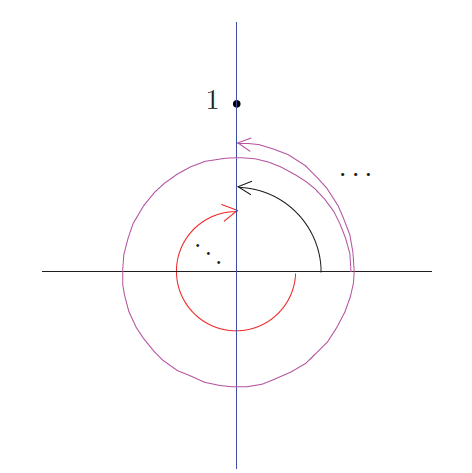
\includegraphics[width=0.4\textwidth]{./Solution/figs/fig-5-11}
\end{center}
\caption{$\cos y + i\sin y = i$를 만족하는 $y$는
$y = \dfrac\pi2 + 2\pi k$ ($k\in \mathbb Z$)로 주어진다.
}
\label{fig-5-11}
\end{figure}

$\exp z = \pi i$라면,
\[
z\in \left\{ \log \pi + i \left(\dfrac\pi 2 + 2\pi k\right) \,:\, k\in\mathbb Z\right\}.
\]
역으로 어떤 $k\in\mathbb Z$에 대하여
$z\in \log \pi + i \left(\dfrac\pi 2 + 2\pi k\right)$라면,
\[
\exp z = e^{\log \pi} \left(
\cos\left(\dfrac\pi2+2\pi k\right) + i \sin\left(\dfrac\pi2+2\pi k\right)
\right) = \pi(0+i\cdot 1) = \pi i.
\]
결론적으로 $\exp z = \pi i$일 필요충분조건은
$z\in \left\{ \log \pi + i \left(\dfrac\pi 2 + 2\pi k\right) \,:\, k\in\mathbb Z\right\}$.

\subsection*{연습문제 \ref{ex-1-33}}

$\gamma(t):= \exp(it)$, $t\in[0,2\pi]$라고 하자. 그러면,
\[
\gamma(t) = \exp(it) = e^0\left(\cos t + i\sin t\right) 
= \cos t + i\sin t.
\]

점 $(\cos t, \sin t)$는 중심이 $(0,0)$이고 반지름이 $1$인 원 위에 있고
$t$가 증가함에 따라 반시계방향으로 움직인다.
따라서 곡선 $t\mapsto \gamma(t)$는 반시계방향으로 도는 원이 된다.
그림 \ref{fig-5-12}\를 참고하라.

\begin{figure}[h!]
\begin{center}
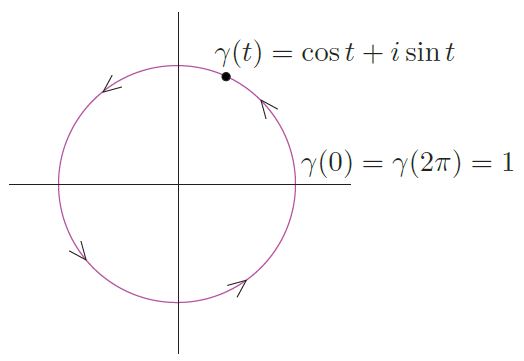
\includegraphics[width=0.35\textwidth]{./Solution/figs/fig-5-12}
\end{center}
\caption{곡선 $t\mapsto \gamma(t):=\exp(it)$, $t\in[0,2\pi]$
}
\label{fig-5-12}
\end{figure}

\subsection*{연습문제 \ref{ex-1-34}}

$\exp(t+it) = e^t(\cos t + i\sin t)$이므로
곡선은 $t\mapsto (e^t\cos t, e^t\sin t)$로 주어진다.
대강의 그림을 그려보면 \ref{fig-5-13}\와 같다.
나선형 곡선이 되며, $t\searrow -\infty$일 때
$(e^t\cos t, e^t\sin t)$는 $0$으로 수렴하고,
$t\nearrow +\infty$일 때 나선형의 바깥으로 발산한다.

\begin{figure}[h!]
\begin{center}
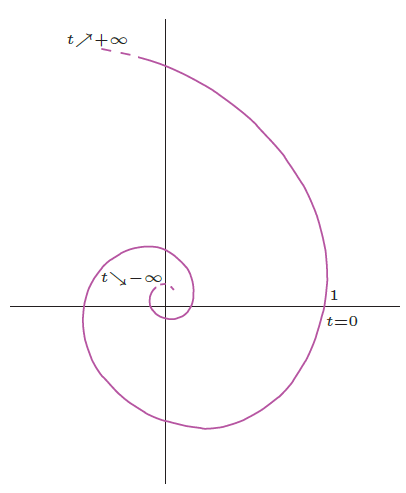
\includegraphics[width=0.3\textwidth]{./Solution/figs/fig-5-13}
\end{center}
\caption{함수 $z=x+iy \mapsto \exp z$에 의한 직선 $y=x$의 상
}
\label{fig-5-13}
\end{figure}

\subsection*{연습문제 \ref{ex-1-35}}

\[
\exp(z^2) = \exp\left( (x+iy)^2 \right)
= \exp(x^2-y^2 + 2xyi) = e^{x^2-y^2}( \cos(2xy) + i \sin (2xy))
\]
이므로
$|\exp(z^2)| = e^{x^2-y^2}$, $\Re(\exp(z^2)) = e^{x^2-y^2} \cos(2xy)$,
$\Im(\exp(z^2)) = e^{x^2-y^2} \sin(2xy)$이다.

$z\ne0$에 대하여
\begin{align*}
\exp \dfrac1z &= \exp\left(\dfrac1{x+iy}\right)
= \exp\left( \dfrac{x-iy}{x^2+y^2} \right) \\
&= e^{\frac{x}{x^2+y^2}} \left( \cos \left( \dfrac{-y}{x^2+y^2} \right)
+i  \sin \left( \dfrac{-y}{x^2+y^2} \right) \right)
\end{align*}
이므로
\begin{align*}
\left| \exp \dfrac1z \right| &= e^{\frac{x}{x^2+y^2}}, \\
\Re\left( \exp \dfrac1z \right) 
& = e^{\frac{x}{x^2+y^2}} \cos \left( \dfrac{-y}{x^2+y^2} \right), \\
\Im\left( \exp \dfrac1z \right) 
&=  e^{\frac{x}{x^2+y^2}} \sin \left( \dfrac{-y}{x^2+y^2} \right).
\end{align*}

\subsection*{연습문제 \ref{ex-1-36}}

$z_1, z_2 \in \mathbb C$에 대하여,
\begin{align*}
(\sin z_1)(\cos z_2) &+ (\cos z_1)(\sin z_2) \\
&= \left( \dfrac{\exp(iz_1) - \exp(-iz_1)}{2i}\right)
\left( \dfrac{\exp(iz_2) + \exp(-iz_2)}{2}\right) \\
&\qquad + \left( \dfrac{\exp(iz_1) + \exp(-iz_1)}{2}\right) 
\left( \dfrac{\exp(iz_2) - \exp(-iz_2)}{2i}\right) \\
&= \dfrac{2\exp(i(z_1+z_2)) -2\exp(-i(z_1+z_2))}{4i}
= \sin(z_1+z_2).
\end{align*}

\subsection*{연습문제 \ref{ex-1-37}}

$z=x+iy$ ($x,y\in\mathbb R$)이라 하면,
\begin{align*}
\cos z &= \cos(x+iy) = (\cos x)(\cos(iy)) - (\sin x)(\sin(iy)) \\
&= (\cos x)\left( \dfrac{e^{-y}+e^y}2\right)
- (\sin x)\left( \dfrac{e^{-y}-e^y}{2i}\right) \\
&= (\cos x)(\cosh y) - (\sin x)\left(-\dfrac{\sinh y}i\right) \\
&= (\cos x)(\cosh y) - i(\sin x)(\sinh y).
\end{align*}
따라서
\begin{align*}
|\cos z|^2 &= (\cos x)^2(\cosh y)^2 + (\sin x)^2(\sinh y)^2 \\
&= (1-(\sin x)^2)(\cosh y)^2 + (\sin x)^2\left(\dfrac{e^{2y} -2 + e^{-2y}}4\right) \\
&= (\cosh y)^2  - (\sin x)^2(\cosh y)^2 + (\sin x)^2
\left(\dfrac{e^{2y} + 2 + e^{-2y}}4 -1\right) \\
&= (\cosh y)^2  - (\sin x)^2(\cosh y)^2 + (\sin x)^2((\cosh y)^2-1) \\
&=  (\cosh y)^2  - \cancel{(\sin x)^2(\cosh y)^2} + \cancel{(\sin x)^2(\cosh y)^2}
-(\sin x)^2 \\
&= (\cosh y)^2 - (\sin x)^2.
\end{align*}

\subsection*{연습문제 \ref{ex-1-38}}

$z=x+iy$ ($x,y\in\mathbb R$)이라 하면,
$\cos z =3$은 다음과 동치이다.
\begin{align}
(\cos x)(\cosh y) &= 3, \label{eq-5-15} \\
(\sin x)(\sinh y) &= 0. \label{eq-5-16}
\end{align}

여기서 $\sinh y=0$는 $y=0$와 동치이다. 
그런데 $y=0$는 불가능하다.
왜냐하면, $z=x+iy=x$가 실수가 되는데 $\cos x =3$을 만족하는 실수 $x$는 없기 때문이다.
그러므로 식 \eqref{eq-5-16}에서 $\sin x = 0$이다.
따라서 $x \in \{ n\pi \,:\, n\in\mathbb Z\}$.
한편, $\cos x = \pm 1$이고, 모든 $y\in\mathbb R$에 대하여
\[
\cosh y = \dfrac{e^y + e^{-y}}2 > 0
\]
이므로 식 \eqref{eq-5-15}에서 $\cos x$는 $-1$이 될 수 없다.
결론적으로 $x \in \{ 2n\pi \,:\, n\in\mathbb Z\}$이고 $\cos x =1$이다.
이제 $\cosh y = 3$에서
\[
\dfrac{e^y + y^{-y}}2 = 3.
\]
즉, $(e^y)^2 - 6e^y+1=0$.
\[
e^y = \dfrac{6\pm \sqrt{36-4}}2 = 3 \pm \sqrt{9-1} = 3\pm 2\sqrt{2}
\]
에서 $y=\log(3+2\sqrt{2})$ 또는 
\[
y=\log(3-2\sqrt{2}) = \log\dfrac{9-8}{3+2\sqrt{2}} = \log \dfrac1{3+2\sqrt{2}} 
= -\log(3+2\sqrt{2})
\]
이므로
$z \in \{ 2\pi n \pm i \log(3+2\sqrt{2}) \,:\, n\in\mathbb Z\}$.

역으로, 어떤 $n\in\mathbb Z$에 대하여 $z=2\pi n \pm i \log(3+2\sqrt{2})$라면,
\begin{align*}
\cos z &= \underbrace{(\cos(2\pi n))}_{=1} \Big(\cosh (\pm \log(3+2\sqrt{2}))\Big)
- i \underbrace{(\sin(2\pi n))}_{=0}(\sinh \cdots)) \\
&= \cosh(\pm \log(3+ 2\sqrt{2})) = \dfrac{e^{\log(3+2\sqrt{2})}+ e^{-\log(3+2\sqrt{2})}}2 \\
&= \dfrac{3+2\sqrt{2} + (3+2\sqrt{2})^{-1}}2 =
\dfrac{3+2\sqrt{2} + 3-2\sqrt{2}}2 = 3.
\end{align*}
종합하면, $\cos z =3$일 필요충분조건은
$z \in \{ 2\pi n \pm i \log(3+2\sqrt{2}), n\in\mathbb Z\}$이다.

\subsection*{연습문제 \ref{ex-1-39}}

\begin{figure}[h!]
\begin{center}
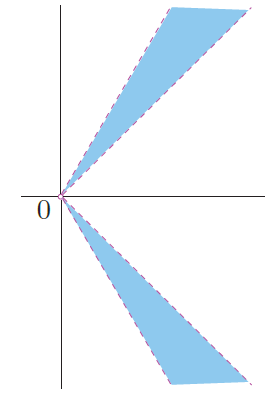
\includegraphics[width=0.25\textwidth]{./Solution/figs/fig-5-14}
\end{center}
\caption{$\left\{ z \in\mathbb C \,:\, z\ne0, \dfrac\pi4 < |\Arg(z)| < \dfrac\pi3 \right\}$
}
\label{fig-5-14}
\end{figure}

\subsection*{연습문제 \ref{ex-1-40}}

\begin{align*}
\Log(1+i) &= \Log\left( \sqrt{2} \left( \dfrac1{\sqrt{2}} + i \dfrac1{\sqrt{2}} \right)\right)
= \Log\left( \sqrt{2} \left( \cos\dfrac\pi4 + i \sin\dfrac\pi4 \right)\right) \\
&= \Log\left(\sqrt{2}\exp\left(i \dfrac\pi4\right)\right) = \log\sqrt{2} + i \dfrac\pi4.
\end{align*}

\subsection*{연습문제 \ref{ex-1-41}}

\begin{align*}
\Log(-1) &= \Log(1\cdot \exp(i\pi)) = \log1 +i\pi = 0 + i\pi = i\pi, \\
\Log(1) &= \Log(1\cdot \exp(i0)) = \log 1 + i0 = 0 + i0 = 0.
\end{align*}
$z=-1$이면,
$\Log(z^2) = \Log((-1)^2) = \Log(1) = 0$인 반면,
$2\cdot\Log(z) = 2\cdot \Log(-1) = 2\cdot i\pi$. 
따라서 $z=-1$일 때,
\[
\Log(z^2) = 0 \ne 2\cdot i\pi = 2\cdot \Log(z).
\]

\subsection*{연습문제 \ref{ex-1-42}}

$\mathbb A:= \{ z \in \mathbb C \,:\, 1 < z < e \}$라 하면,
$z\in \mathbb A$일 필요충분조건은 $ z=r\exp(i\Arg(z))$이고
$1<r<e$, $\Arg(z)\in (-\pi,\pi]$이다.
이런 $z$에 대하여
\[
\Log(z) = \Log(r\exp(i\Arg(z))) = \log r + i\Arg(z)
\]
이고 $0=\log 1 < \log r < \log e = 1$이다.
따라서 상은 직사각형
\[
\mathbb I := \{ x+iy\,:\, 0<x<1, -\pi <y\le \pi \}
\]
가 된다.

\begin{figure*}[h!]
\begin{center}
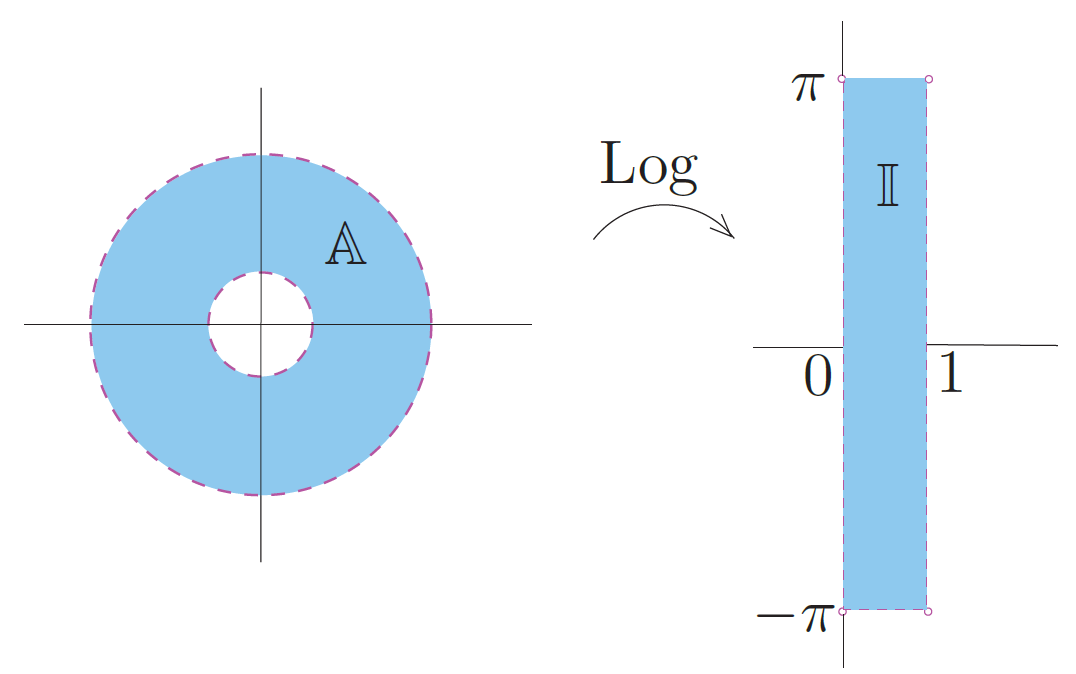
\includegraphics[width=0.45\textwidth]{./Solution/figs/fig-s-0-5}
\end{center}
%\caption{$\left\{ z \in\mathbb C \,:\, z\ne0, \dfrac\pi4 < |\Arg(z)| < \dfrac\pi3 \right\}$}
%\label{fig-5-14}
\end{figure*}

역으로, $x+iy\in\mathbb I$이면,
$z:= \exp(x+iy) = e^x\exp(iy)\in \mathbb A$이다.
왜냐하면, $|z|=e^x \in (1,e)$이고 
$\Arg(z) = y$는 $(-\pi,\pi]$ 범위에 있다.
%$\Log(z) = \Log (e^x \exp(iy)) = \log e^x + iy = x+iy$이기 때문이다.
따라서 $\mathbb A$의 $\Log$함수에 대한 상은 정확히 $\mathbb I$와 일치한다.

\subsection*{연습문제 \ref{ex-1-43}}

$(1+i)^{1-i}$의 주치는 $\exp((1-i)\Log(1+i))$이다.
\[
\Log(1+i)  = \Log \left( \sqrt{2}\exp\left(i \dfrac\pi4\right)\right)
= \log\sqrt{2} + i \dfrac\pi4.
\]
따라서 $(1+i)^{1-i}$의 주치를 계산하면,
\begin{align*}
\exp((1-i)\Log(1+i)) &= \exp\left( (1-i)\left(\log\sqrt{2} + i \dfrac\pi4\right)\right) \\
&= e^{\log\sqrt{2} + \frac\pi4} \exp \left( i\left( \dfrac\pi4 - \log\sqrt{2} \right)\right) \\
&= \sqrt{2} e^{\frac\pi4} \dfrac{(1+i)}{\sqrt{2}} \exp\left(-i\log\sqrt{2}\right) \\
&=e^{\frac\pi4}(1+i)\left(\cos (\log\sqrt{2}) - i \sin(\log\sqrt{2})\right).
\end{align*}













